% this file is called up by thesis.tex
% content in this file will be fed into the main document
\ifpdf
    \graphicspath{{2/figures/PNG/}{2/figures/PDF/}{2/figures/}}
\else
    \graphicspath{{2/figures/EPS/}{2/figures/}}
\fi
\chapter{Technologie} % top level followed by section, subsection


% ----------------------- contents from here ------------------------

\section{Apache ServiceMix}
Integracja systemów informatycznych jest jednym z największych wyzwań stojących przed nowoczesnymi przedsiębiorstwami. Apache ServiceMix pomaga rozwiązać ten problem będąc bazującym na standardach, lekkim oraz stosującym paradygmat "luźnego powiązania" narzędziem. Dzięki bazowaniu na standardach w sposób drastyczny zmniejsza szanse na uzależnienie się od konkretnego dostawcy oprogramowania, przez sotowanie luźnego-powiązania zmniejsza złożoność integracji. 
Jest to otwarta implementacja ESB, zbudowana w oparciu o JBI i wydana na licencji Apache, od wersji 4 ServiceMix wykorzystuje OSGi do uproszczenia podziału aplikacji na komponenty. 	
Architekturę ServiceMix'a można podzielić na 3 warstwy:
\begin{enumerate}
	\item Warstwa jądra
	\item Warstwa serwisów
	\item Warstwa aplikacji
\end{enumerate}  
\newpage
\begin{figure}[!h]
	\centering
	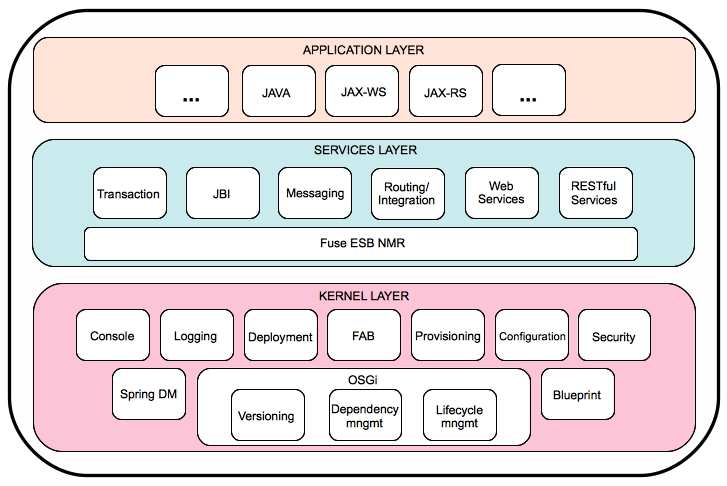
\includegraphics[scale=0.45]{ServiceMixArchitektura.jpg} 
	\caption{Architektura ServiceMix 4}
\end{figure}
Każda z tych warstw ma inne zadania i odpowiada za inne czynności.
\begin{itemize}
	\item Warstwa jądra - bazuje na Apache Karaf czyli implementacji OSGi będącą lekkim kontenerem do którego można wdrożyć różne komponenty i aplikacje. Warstwa ta wspólpracuje z warstwą serwisów w celu stworzenia, skoordynowania, utrzymania i zarządzania logowaniem, bezpieczeństwem oraz transakcjami. Najważniejsze funkcje dostarczane przez tą warstwę to:
	\begin{itemize}
		\item Osadzanie - umożliwia zarówno manualne jak i automatyczne osadzanie bibliotek
		\item Kontener OSGi - ServiceMix 4 wspiera 2 różne kontenery OSGi a mianowicie Eclipse Equinox i Apache Felix
		\item Wstrzykiwania zależnośći - wykorzystuje 2 różne frameworki:
			\begin{itemize}
				\item Blueprint
				\item Spring DI
			\end{itemize}   
		\item Automatyczna konfiguracja - dokonując zmian w pliku z właściwościami można dokonać zmian "w locie", bez restartowania serwera
		\item Bezpieczeństwo - framework odpowiadający za bezpieczeństwo bazuje na JAAS, dostarcza kilka różnych, odizolowanych poziomów:
			\begin{itemize}
				\item kontenera OSGi
				\item wbudowanej instancja serwisu wiadomości
				\item osadzonych instancji serwisow router'a i integracyjnego
			\end{itemize} 
		\item Logowanie - dynamiczne logowanie wspierające różne interfejsy takie jak: JCL, SLF4J, Avalon, łatwo konfigurowalne poprzez pliki z właściwościami
		\item Konsola - umożliwia zarządzanie i pełną kontrolę nad cała aplikacją
	\end{itemize}  
	\item Warstwa serwisów - 	składa się z interfejsów i klas reprezentujących wbudowane serwisy. Współpracuje z warstwą aplikacji w celu komunikacji z aplikacjami użytkowników które chcą korzystać z oferowanych serwisów. Najważniejsze funkcje dostarczane przez tą warstwę to:
	\begin{itemize}
		\item Rutowanie i integracja - bazuje na Apache Camel, umożliwia zdefiniowanie ścieżek i zaimplementowanie biznesowych wzorców w celach integracji a następnie osadzenie jako paczka OSGi
		\item Tworzenie serwisów webowych - bazzuje na Apache CXF, umożliwia, w prosty sposób, tworzenie i osadzanie jako paczka OSGi serwisów webowych implementujących API JAX-WS 
		\item Tworzenie serwisów RESTful'owych - bazuje na Apache CXF, umożliwia w prosty sposób, tworzenie i osadazanie jako paczka OSGi serwisów RESTful'owych implementujących API JAX-RS
		\item Tworzenie i osadzanie jednostek i zespołów serwisów bazujących na JBI
		\item Komunikacje - udostępnia serwis wiadomości w całości zbudowany na Apache ActiveMQ, umożliwiający tworzenie i osadzanie zarówno klientów jak i nadawców wiadomości JMS
		\item Menadżer transakcji - bazuje na Apache Aries, wystawia interfejs transakcji jako serwis, umożliwia tworzenie i osadzanie zarówno aplikacji bazujących na framework'u JTA jak i na Spring'u
		\item Znormalizowany ruter wiadomości - jego główną rolą jest przekazywanie wiadomości pomiędzy różnymi aplikacjami osadzonymi w kontenerze OSGi oraz, jeżeli zachodzi taka konieczność, pomiędzy aplikacjami z OSGi a aplikacjami osadzonymi w kontenerze JBI
	\end{itemize}
	\item Warstaw aplikacji - w tym miejscu znajdując się aplikacje użytkownika, ServiceMix 4 dostarcza wielu różnych API(częściowo wymienionych w warstwie serwisów) za pomocą których aplikacje klienckie mogą łączyć się i korzystać z usług oferowanych przez serwisy działające wewnątrz kontenera
\end{itemize}

\section{IvonaTTS}
Głównym wyzwaniem stawianym przed syntezatorami mowy jest czytanie tekstu w sposób naturalny, głosem możliwie jak najbardziej podobnym do ludzkiego. Pomimo dużego postępu jaki dokonał się w tej dziedzinie w ciągu ostatnich lat, głosy oferowane przez współczesne syntezatory wciąż brzmią sztucznie, czyniąc słuchanie ich bez zmęczenia zadaniem dość trudny. IvonaTTS wykorzystuje dwie autorskie technologie, mianowicie:
\begin{itemize}
	\item BrightVoices
	\item Rapid Voice Development
\end{itemize} 
BrightVoices zapewniaja ekspresyjne, wyraziste, czyste, lektorskie brzmienie zarówno słów, zdań czy nawet całych książek. Jest ona efektem przeszło 10-letnich badań naukowych. Technologia ta korzysta z nowoczesnych algorytmów z dziedziny sztucznej inteligencji, umożliwiają one precyzyjne odzwierciedlanie ekspresji oraz różnych, nieraz bardzo indywidualnych, cech ludzkiego głosu.   \\
Rapid Voice Development w sposób znaczny przyspiesza proces tworzenia ludzkiego głosu. Pozwala także na efektywne, szybkie i precyzyjne rozpoznawianie sygnałów mowy w nagraniach lektorskich. Wszystko to jest możliwe do osiągnięcia dzięki doskonałemu modelowaniu zagadnień językowych takich jak:
\begin{itemize}
	\item akcentowanie,
	\item fonetyzacja,
	\item artykulacja,
	\item intonacja.
\end{itemize}
Według niezależnej amerykańskiej organizacji Voice Information Assiociates syntezator IvonaTTS jest najdokładniejszym spośród dostępnych na rynku komercyjnych syntezatorów. Pozostawia w tyle produkty takich firm jak Microsoft, Nuance, Loquendo czy AT\&T.
\begin{figure}[!h]
	\centering
	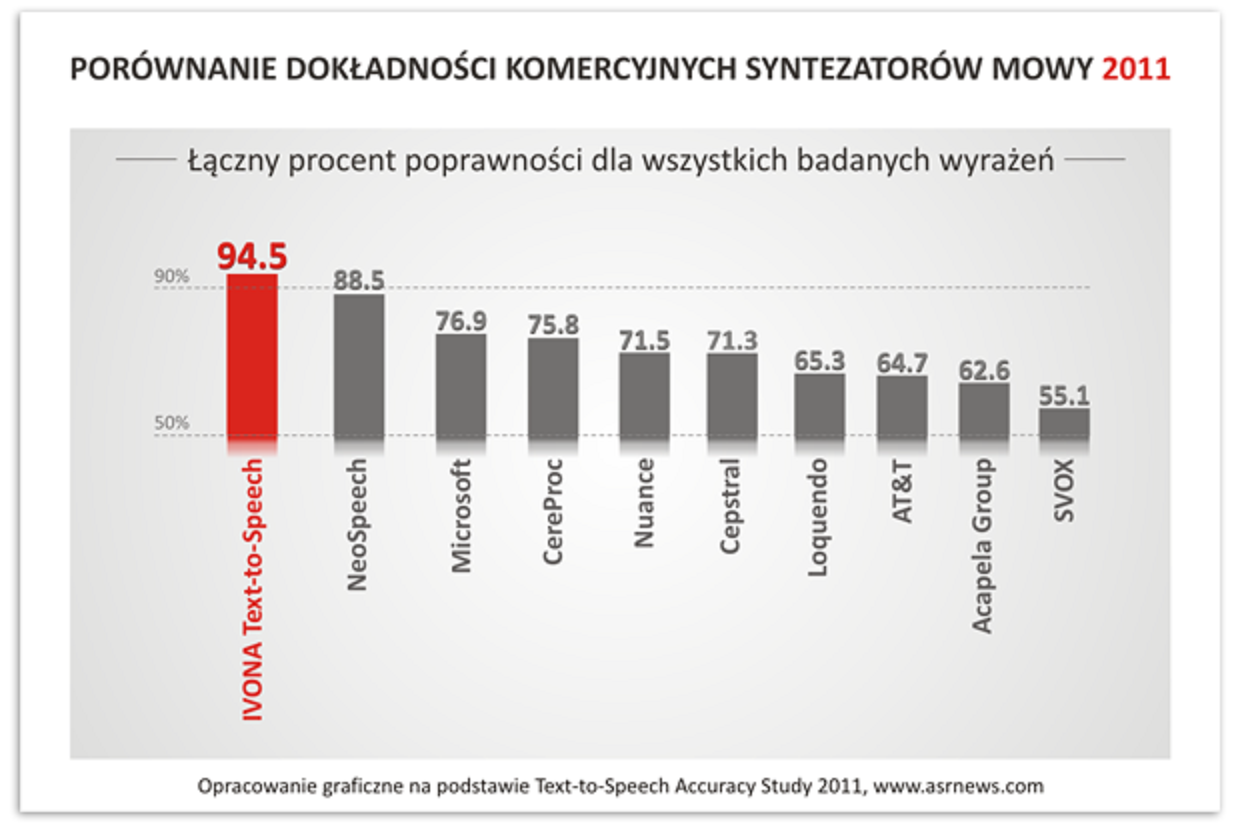
\includegraphics[scale=0.45]{IvonaWydajnosc.png} 
	\caption{Dokładność IvonaTTS w porównaniu do konkurencji}
\end{figure}



% ---------------------------------------------------------------------------
% ----------------------- end of thesis sub-document ------------------------
% ---------------------------------------------------------------------------